\documentclass[handout]{beamer}  %%% FÜR HANDOUT ALS PDF

\setbeamertemplate{navigation symbols}{}
\usetheme{Madrid}
\usecolortheme{seagull}
\beamersetuncovermixins{\opaqueness<1>{10}}{\opaqueness<2->{15}}
\usepackage[english]{babel}
\usepackage{csquotes}
\usepackage{graphicx}
\usepackage{verbatim}
\newcounter{saveenumi}
\newcommand{\seti}{\setcounter{saveenumi}{\value{enumi}}}
\newcommand{\conti}{\setcounter{enumi}{\value{saveenumi}}}
\usepackage[hyperref=true,style=authoryear, dashed=false, maxnames=3,backend=bibtex8,doi=false,isbn=false,backref=true]{biblatex}
\usepackage{amssymb,amsmath}
%\setlength{\bibitemsep}{\baselineskip}
\usepackage{xcolor}
\usepackage{graphicx,pstricks,beamerprosper}
\usepackage{subfigure}
\usepackage{verbatim}


\begin{document}
\author[Willi Mutschler]{Willi Mutschler, M.Sc.}
\date{Summer 2015}
\institute[Institute of Econometrics]{Institute of Econometrics and Economic
Statistics\\University of M\"unster\\willi.mutschler@wiwi.uni-muenster.de}
\title[DSGE methods]{PhD Macroeconomics - DSGE methods}

\begin{frame}
\titlepage
\end{frame}

\begin{frame}\frametitle{Previously\dots}
\begin{itemize}[<+->]
  \item Theory and intuition behind baseline DSGE models
  \item Derivation of the structural form, log-linearization and solution via method of undetermined coefficients
\begin{block}{Insight}
DSGE model consists of
\begin{itemize}
     \item set of Euler equations, i.e. first-order optimality conditions,
     \item transition equations for state and control variables
     \item transition equations for structural shocks and innovations,
     \item observable variables and measurement errors
\end{itemize}
which can be cast into a nonlinear system of expectational difference equations.
\end{block}
\end{itemize}
\end{frame}

\begin{frame}
	\frametitle{Introduction to Dynare}\framesubtitle{}
	Dynare
	\begin{itemize}
		\item computes the solution of deterministic models (arbitrary accuracy)
		\item computes first, second and third order approximation to solution of stochastic models
		\item estimates (maximum likelihood or Bayesian approach) parameters of DSGE models
		\item computes optimal policy
		\item performs global sensitivity analysis of a model
		\item solves problems under partial information
		\item estimates BVAR and Markov-Switching Bayesian VAR models
		\item estimates DSGE-VAR models
		\item estimates Markov-Switching DSGE models
		\item \dots
	\end{itemize}
\end{frame}

\section{General DSGE framework}

\begin{frame}
	\frametitle{\secname}
	
	\begin{block}{General DSGE model}
		\begin{align*}
		0 &=   E_t f \left( x_{t+1},y_{t+1},x_t,y_t|\theta \right),\\
		x_{t+1}  &= h(x_{t},\varepsilon_{t+1}|\theta),\\
		y_{t+1} &= g(x_t,\varepsilon_{t+1}|\theta) ,\\
		d_t &= D y_t+  \mu_{t}.
		\end{align*}
		with $E(\varepsilon_t)=0$, $E(\varepsilon_t\varepsilon_t')=\Sigma_\varepsilon$ and $E(\mu_t)=0$, $E(\mu_t\mu_t')=\Sigma_\mu$.
	\end{block}
	Some remarks
	\begin{itemize}
		\item  DSGE-models can be interpreted as \emph{state-space-models}.
		\item Driving force of the model are exogenous shocks and innovations $\varepsilon_t$.
		\item Stability and determinacy: Check Blanchard and Khan conditions
		\item Flexible framework: you can add auxiliary variables and equations.
	\end{itemize}
\end{frame}


\begin{frame}\frametitle{Deterministic vs. Stochastic models}
	\begin{itemize}
		\item Major distinction: Are future shocks known?
		\begin{itemize}
			\item Deterministic models: occurrence of all future shocks is known exactly at the time of computing the model's solution
			\item Stochastic models: only the distribution of future shocks is known			
		\end{itemize}
\item If you have a linear model or first order linear approximation of the stochastic model the two cases become practically the same, due to certainty equivalence.			
	\end{itemize}
\end{frame}
\note{Let's consider a shock to a model's innovation only in period 1. In a deterministic context, agents will take their decisions knowing that future values of the innovations will be zero in all periods to come. In a stochastic context, agents will take their decisions knowing that the future value of innovations are random but will have zero mean. This isn't the same thing because of Jensen's inequality.\\
A second order approximation will instead lead to very different results, as the variance of shocks will matter.}

\begin{frame}\frametitle{Deterministic vs. Stochastic models}
Deterministic models useful for
		\begin{itemize}
			\item Models with full information, perfect foresight and no uncertainty around shocks.
			\item Focus on impact of a change in regime, e.g. introduction of a new tax
			\item Shocks can hit today or at any time in the future, in which case they would be expected with perfect foresight. They can also last	one or several periods.
			\item Most often, though, models introduce a positive shock today and zero shocks thereafter (with certainty).
			\item Solution does not require linearization, but numerical simulation techniques to find the	exact paths of endogenous variables that meet the model
			\item In practice useful to get a first glimpse of model before using the stochastic model for further analysis and estimation
		\end{itemize}
\end{frame}

\begin{frame}\frametitle{Deterministic vs. Stochastic models}
Stochastic models useful for
		\begin{itemize}
			\item 	More popular in literature: RBC models or new keynesian monetary models.
			\item Shocks hit today (with a surprise), but thereafter their expected value is zero. Expected future shocks, or permanent changes in the exogenous variables cannot be handled due to the use of Taylor approximations around a steady state.
			\item Note that when these models are linearized to the first order, agents behave as if future shocks where equal to zero (since their expectation is null), which is the certainty equivalence property.
			\begin{itemize}
				\item This does NOT mean that model is deterministic
			\end{itemize}
		\item Useful for estimation!
		\end{itemize}
		
\end{frame}

\section{DSGE solution}
\begin{frame}
	\frametitle{\secname}
	One distinguishes between linear and non-linear methods:
	\begin{itemize}
		\item Linear methods: Anderson/Moore (1983), Binder and Pesaran, Blanchard/Khan (1980),
		(1997), Christiano (2002), King and Watson (1998), Klein (2000), Sims (2001) and Uhlig (1999) (See Anderson (2008) for a comparison).
		\item Nonlinear methods: Projection methods, iteration procedures or perturbation approach (see DeJong/Dave (2011) for a comparison)
	\end{itemize}
	Dynare uses the perturbation approach:
	\begin{itemize}
		\item Perturbation approach finds a \underline{local} approximation of the policy functions in a neighborhood of a particular point
		\item Mostly steady-state, since we can solve it analytically or numerically.
	\end{itemize}
\end{frame}

\begin{frame}
	\frametitle{\secname}\framesubtitle{First-order approximation}
	\textbf{Pros}:
	\begin{itemize}
		\item Simple linear state-space representation of the model, which in many cases is sufficiently exact.
		\item One can use the Kalman-filter to empirically evaluate the system.
	\end{itemize}
	\textbf{Cons}:
	\begin{itemize}
		\item One looses important information during the linearization.
		\item Higher moments play an important role for analyzing markets, risk, welfare, etc.
		\item An approximation to, say, the second order can yield different results, because the variance of future shocks matters (risk premium).
	\end{itemize}
	
\end{frame}





\begin{frame}
	\frametitle{Certainty-equivalence}
	Important theoretical result for stochastic models:
	\begin{itemize}
		\item Even though agents take the effect of future shocks into account when optimizing, in a linearization to the first-order they don't matter for the decision rule.
		\begin{block}{\emph{Certainty-equivalence-property}}
			\begin{itemize}
				\item In a first-order approximation the constant term needs not to be corrected for uncertainty (i.e. variance of shocks)
				\item Expectation of $x_t$ and $y_t$ is equal to its non-stochastic steady-state
			\end{itemize}
		\end{block}
		\item This is problematic when uncertainty does matter: risk premia, welfare evaluation, \dots
	\end{itemize}
\end{frame}




\begin{frame}
  \frametitle{Toy example: Clarida-Gali-Gertler}\framesubtitle{Household}\footnotesize
Household preferences are given by
\begin{equation*}
E_{0}\sum_{t=0}^{\infty }\left( \log C_{t}-\exp \left( \tau _{t}\right)
\frac{N_{t}^{1+\varphi }}{1+\varphi }\right) ,\qquad \tau_{t}=\lambda \tau_{t-1}+\varepsilon_{t}^{\tau },\qquad \varepsilon_{t}^{\tau }\sim iid.
\end{equation*}
\begin{itemize}
\item $C_{t}$ denotes consumption,
\item $\tau_{t}$ denotes a time preference shock,
\item $N_{t}$ denotes employment,
\item $\varphi$ denotes a labor supply parameter.
\end{itemize}
The budget constraint of the household is
\begin{equation*}
  P_{t}C_{t}+B_{t+1}\leq W_{t}N_{t}+R_{t-1}B_{t}+T_{t},
\end{equation*}
\begin{itemize}
  \item $T_t$ denotes (lump-sum) taxes and profits,
  \item $P_t$ denotes price level,
  \item $W_t$ denotes nominal wage rate
  \item $B_{t+1}$ denotes bonds purchased at time $t$, which deliver a non-state-contingent rate of return, $R_{t}$, in period $t+1.$
\end{itemize}
\end{frame}

\begin{frame}    \frametitle{Toy example: Clarida-Gali-Gertler}\framesubtitle{Competitive firms}
Competitive firms produce a homogeneous output good, $Y_{t},$ using the following technology:
\[
Y_{t}=\left[ \int_{0}^{1}Y_{i,t}^{\frac{\varepsilon -1}{\varepsilon }}\right]
^{\frac{\varepsilon }{\varepsilon -1}}di,\text{ }\varepsilon >1,
\]%
\begin{itemize}
\item $Y_{i,t}$ denotes the $i^{th}$ intermediate good, $i\in \left(0,1\right).$
\end{itemize}
Competitive firms take the price of the final output good, $P_{t},$ and the prices of the intermediate goods, $P_{i,t},$ as given and choose $Y_{t}$ and $Y_{it}$ to maximize profits;
\[
Y_{i,t}=Y_{t}\left( \frac{P_{t}}{P_{i,t}}\right) ^{\varepsilon }.
\]%
\begin{itemize}
  \item This is the demand curve for the producer of $Y_{it}$ in the intermediate sector.
\end{itemize}
\end{frame}

\begin{frame}    \frametitle{Toy example: Clarida-Gali-Gertler}\framesubtitle{Intermediate firms}
The $i^{th}$ intermediate good firm is a monopolist for $Y_{it}$ and uses labor, $N_{i,t},$
to produce output using the following production function:%
\[
Y_{i,t}=\exp \left( a_{t}\right) N_{i,t},\text{ }\Delta a_{t}=\rho \Delta
a_{t-1}+\varepsilon _{t}^{a},
\]%
\begin{itemize}
  \item $\Delta $ is the first difference operator,
  \item $\varepsilon _{t}^{a}$ is an iid shock $\rightarrow$ $a_{t}$ has a unit root representation
\end{itemize}
The $i^{th}$ firm sets prices subject to Calvo frictions. In particular,%
\[
P_{i,t}=\left\{
\begin{array}{cc}
\tilde{P}_{t} & \text{with probability }1-\theta \\
P_{i,t} & \text{with probability }\theta%
\end{array}%
\right. ,
\]%
\begin{itemize}
  \item $\tilde{P}_{t}$ denotes the price chosen by the $1-\theta $ firms that can reoptimize their price at time $t.$
\end{itemize}
\end{frame}

\begin{frame}
\frametitle{Toy example: Clarida-Gali-Gertler}\framesubtitle{Intermediate firms}
\begin{itemize}
  \item The $i^{th}$ producer is competitive in labor markets, pays $W_{t}\left( 1-\nu \right)$ for one unit of labor.
  \item $\nu $ represents a subsidy which eliminates the monopoly distortion on labor in the steady state:
  $$1-\nu=\left( \varepsilon -1\right) /\varepsilon .$$
\end{itemize}
\end{frame}

\begin{frame}\frametitle{Toy example: Clarida-Gali-Gertler}\framesubtitle{Ramsey equilibrium}
The Ramsey equilibrium for the model is the equilibrium associated with the
optimal monetary policy, it is characterized by
\begin{itemize}
  \item zero inflation, $\pi _{t}=0,$ at each date and for each realization of $a_{t}$ \& $\tau _{t}$
  \item consumption and employment correspond to their first best levels
  \item $C_{t}$ and $N_{t}$ satisfy the resource constraint
\[
C_{t}=\exp \left( a_{t}\right) N_{t},
\]
\item marginal rate of substitution between consumption
and labor equals the marginal product of labor%
\[
\frac{\text{marginal utility of leisure}}{\text{marginal utility of
consumption}}=C_{t}\exp \left( \tau _{t}\right) N_{t}^{\varphi }=\exp \left(
a_{t}\right) .
\]%
\end{itemize}
\end{frame}

\begin{frame}\frametitle{Toy example: Clarida-Gali-Gertler}\framesubtitle{Ramsey equilibrium}
Solving yields:
\begin{align*}
\pi_t^* &= 0,\\
n^*_t &:= \log \left( N_{t}^{\ast }\right) =-\frac{\tau _{t}}{1+\varphi },\\
c^*_t &:= \log \left( C_{t}^{\ast }\right) =a_{t}-\frac{\tau _{t}}{1+\varphi } = \log\left( Y_{t}^{\ast }\right) =: y^*_t,\\
r_t^* &:= log(R_t^* \beta) =E_{t}\Delta a_{t+1}-E_{t}\frac{\tau _{t+1}-\tau _{t}}{1+\varphi },
\end{align*}
\begin{itemize}
  \item $\ast $ indicates a variable corresponding to the Ramsey equilibrium, i.e. natural rates,
  \item lower case letters are log of the corresponding variable,
  \item $r_t^*$ is log deviation from non-stochastic steady-state.
\end{itemize}
\end{frame}


\begin{frame}\frametitle{Toy example: Clarida-Gali-Gertler}\framesubtitle{The model equations}
Linearizing about the steady-state the model equations are given by\footnotesize
\begin{eqnarray*}
\pi _{t} &=&\beta E_{t}\pi _{t+1}+\kappa x_{t}\text{ (Calvo pricing equation)} \\
x_{t} &=&-\left[ r_{t}-E_{t}\pi _{t+1}-r_{t}^{\ast }\right] +E_{t}x_{t+1}\text{ (intertemporal equation)} \\
r_{t} &=&\alpha r_{t-1}+(1-\alpha )\left[ \phi _{\pi }\pi _{t}+\phi _{x}x_{t}%
\right] \text{ (policy rule)} \\
r_{t}^{\ast } &=&\rho \Delta a_{t}+\frac{1}{1+\varphi }\left( 1-\lambda
\right) \tau _{t}\text{ (natural rate)} \\
\Delta y_t &=& x_{t} - x_{t-1} + \Delta a_t - \frac{\tau_t - \tau_{t-1}}{1+\varphi} \text{  (output growth)}\\
\Delta a_t &=& \rho \Delta a_{t-1} + \varepsilon_{t}^a \text{  (technological shock)}\\
\tau_t &=& \lambda \tau_{t-1} + \varepsilon_{t}^\tau \text{  (preference shock)}
\end{eqnarray*}
and
\begin{align*}
y_{t}^{\ast } &=a_{t}-\frac{1}{1+\varphi }\tau _{t}\text{ (natural output)}\\
x_{t} &=y_{t}-y_{t}^{\ast }\text{ (output gap)}\\
\kappa &= \frac{(1-\theta)(1-\beta \theta) (1+\varphi)}{\theta}
\end{align*}
\end{frame}

\begin{frame}\frametitle{Toy example: Clarida-Gali-Gertler}\framesubtitle{Practicing Dynare}
\begin{enumerate}
  \item Install Matlab and Dynare, open cgg.mod, try to understand the code, run it. Interpret the Dynare output.
  \item Compute the impulse response function of the model to a technology shock for the next 7 periods in both the deterministic as well as stochastic model. Explain the difference or equivalence.
  \item Given the IRF, indicate whether the economy over- or under- responds due to the shocks, relative to their natural response. What is the economic intuition in each case?
  \item Do the calculations with $\phi_\pi=0.99$. Explain the error message and give economic intuition behind this.
\seti\end{enumerate}
\end{frame}

\begin{frame}\frametitle{Toy example: Clarida-Gali-Gertler}\framesubtitle{Practicing Dynare}
Return to $\phi_\pi=1.5$.
\begin{enumerate}\conti
  \item Explain why it is that when the monetary policy rule is replaced by the natural equilibrium, i.e. $r_t =r_t^*$, the solution is indeterminate.
  \item Now replace the monetary policy rule by
  \begin{equation*} r_{t} = r_t^{\ast} + \alpha (r_{t-1}-r^\ast_{t-1})+(1-\alpha )\left[ \phi _{\pi }\pi _{t}+\phi _{x}x_{t}\right]\end{equation*}
  Explain why this Taylor rule uniquely supports the natural equilibrium.\seti
\end{enumerate}
Return to the original Taylor rule. Calibrate the model to a more empirically relevant parametrization: $\phi_x=0.15,\alpha=0.8,\rho=0.9$
\begin{enumerate}\conti
   \item Simulate the model for 1000 periods. Save the middle 100 observations of $dy_t$ and $\pi_t$ into an Excel-file as well as into a mat-file. Plot the path of output growth.
\seti\end{enumerate}
\end{frame}


\begin{frame}\frametitle{Exercise: Write your own MOD file}
	Consider the following simplified RBC-model (social planer problem);
	\begin{align*}
		\underset{\{c_{t+j},\ell_{t+j},k_{t+j}\}_{j=0}^\infty}{max} W_t &= \sum_{j=0}^\infty \beta^j u(c_{t+j},\ell_{t+j})\\
		s.t.\quad y_t &= c_t + i_t, & A_t &= \bar{A}e^{a_t}, \\
		y_t &= A_t f(k_{t-1},\ell_t), & a_t &= \rho a_{t-1} + \varepsilon_t,\\
		k_t &= i_t +(1-\delta)k_{t-1}, &  \varepsilon_t &\sim N(0,\sigma_{\varepsilon}^2),
	\end{align*}
	where preferences and technology follow:
	\begin{align*}
		u(c_t,\ell_t)= \frac{\left[c_t^\theta (1-\ell_t)^{1-\theta}\right]^{1-\tau}}{1-\tau}, \qquad f(k_{t-1},\ell_t)=\left[\alpha k_{t-1}^\psi + (1-\alpha)\ell_t^\psi\right]^{1/\psi}.
	\end{align*}
	Optimality is given by:
	\begin{eqnarray*}
		&u_c(c_t,\ell_t) = \beta E_t \left\{u_c(c_{t+1},\ell_{t+1}) \left[A_{t+1} f_k(k_t, \ell_{t+1})+1-\delta \right]\right\},\\
		& \frac{u_\ell(c_t,\ell_t)}{u_c(c_t,\ell_t)}+A_t f_\ell(k_{t-1},\ell_t)=0,\\
		& c_t + k_t = A_t f(k_{t-1},\ell_t) +(1-\delta)k_{t-1}.
	\end{eqnarray*}
\end{frame}

\begin{frame}[fragile]\frametitle{Exercise: Write your own MOD file}\framesubtitle{Steady-state}
Note that we could either compute the steady-state analytically and then use steady\_state\_model in our mod-file or good guesses for an initval block. If you want to use intival, you can use these values
\begin{verbatim}
k  		 = 20;
y  		 = 1;
l  		 = 0.5;
c  		 = 1.5;
A  		 = 1;
a  		 = 0;
i  		 = 0.5;
uc 		 = 0.5;
ul 		 = -1;
fk 		 = 0.1;
fl 		 = 3;
f  		 = 2;
\end{verbatim}
\end{frame}


\begin{frame}\frametitle{Exercise: Write your own MOD file}\framesubtitle{Calibration}

\begin{tabular}{lcc}
	 Weight of consumption in utility & $\theta$ & 0.357 \\
	 Risk aversion & $\tau$ & 2.0 \\
	 Share of capital in production & $\alpha$  & 0.45 \\
	 Elasticity of substitution capital/labor & $\psi$ & -0.1 \\
	 Discount factor & $\beta$ & 0.99 \\
	 Depreciation rate & $\delta$ & 0.02 \\
	 Autocorrelation of productivity & $\rho$ & 0.8 \\
	 Steady state level of productivity & $A^{*}$ & 1
\end{tabular}
\end{frame}


\begin{frame}[shrink]\frametitle{Exercise: Write your own MOD file}\footnotesize
	\begin{enumerate}[(a)]
		\item Write a mod-file for this model. If your residuals are not 0, you can try different optimizers to find the steady-sate, e.g. steady(solve\_algo=3).
		\item Assume that the economy starts from $k_0=0.5 \bar{k}$. Use a deterministic simulation to show how consumption and capital return to equilibrium. Hint: Use histval block.
		\item Assume that the economy starts from steady state. Use a deterministic simulation to show the effects on consumption and capital of an unexpected 1\% negative shock at the beginning of period 1. Hint: Use shocks block.
		\item Assume that the economy starts from steady state. Use a deterministic simulation to show the effects consumption and capital of favourable pre-announced shocks in the future, i.e. a sequence of positive shocks to $A_t$: 4\% in period 5 and an additional 1\% during the following periods. Hint: Use shocks block.
		\item Assume that the economy starts from steady state. In period 1, TFP increases by 5\% permanently (and this was unexpected). Use a deterministic simulation to show the transition path of consumption and capital in response to this permanent shock. Hint: Use endval block.
		\item Assume that the economy starts from steady state. In period 6, TFP increases by 5\% permanently (and this was expected). Use a deterministic simulation to show the transition path of consumption and capital in response to this pre-announced permanent shock. Hint: Use endval and shock block.
		\item Simulate a sample of 10000 observations for $c_t,\ell_t$ and $y_t$ using \texttt{stoch\_simul} and save it in a mat-file.
	\end{enumerate}
\end{frame}




\section{Overview Estimation-Methods}
\begin{frame}\frametitle{Overview Estimation-Methods}\framesubtitle{}
\begin{itemize}
    \item Econometrically, a DSGE-Model is a state-space model of which
        one has to determine the parameters.
      \item Three concepts:
      \begin{enumerate}
        \item \textbf{Calibration}: The parameters are set in such a
            way, that they closely correspond to some theoretical
            moment or stylized fact of data.
        \item \textbf{Methods of limited information [not covered]} or weak
            econometric interpretation: Minimize the distance between
            theoretical and empirical moments, i.e.
            \emph{General-Method-of-Moments} or \emph{Indirect
            Inference}.
        \item \textbf{Methods of full information} or strong
            econometric interpretation: The goal is an exact
            characterization of observed data, i.e.
            \emph{Maximum-Likelihood} or \emph{Bayesian methods}.
      \end{enumerate}
\end{itemize}
\end{frame}

\section{Calibration}
\begin{frame}\frametitle{Calibration}\framesubtitle{}
\begin{itemize}
   \item Goal: To answer a specific quantitative research question using
       a structural model.
   \item Construct and parameterize the model such, that it corresponds
       to certain properties of the true economy.
   \item Use steady-state-characteristics for choosing the parameters in
       accordance with observed data.
   \item Often: stable long-run averages (wages, working-hours, interest
       rates, inflation, consumption-shares, government-spending-ratios,
       etc.).
   \item You can use micro-studies as well, however, one has to be
       careful about the aggregation!
\end{itemize}
\end{frame}

\subsection{Hints for calibrating a model}
\begin{frame}\frametitle{Calibration}\framesubtitle{Hints for calibrating a model}

\begin{itemize}
   \item Use long-term averages of interest rates, inflation, average
       growth of productivity, etc. for \emph{steady-state} values.
   \item BUT: Weil (1989) shows, that in models with representative
       agents there is an overestimation of \emph{steady-state} interest
       rates (\emph{risk-free rate puzzle}). It is possible that you get
       absurd constellation of parameters, like a discount-factor of
       $\beta>1$.
   \item Usual mark-up on prices is around 1.15 (Corsetti et al (2012)).
   \item Intertemporal elasticity of substitution  $1/\sigma$ somewhere
       between $\sigma=1$ and $\sigma=3$ (King, Plosser and Rebelo
       (1988), Rotemberg and Woodford (1992), Lucas (2003)).
\end{itemize}
\end{frame}

\begin{frame}\frametitle{Calibration}\framesubtitle{Hints for calibrating a model}
\begin{itemize}
   \item Rigidity of prices: For an average price adjustment of 12-15
       months see Keen and Wang (2007).
   \item Coefficients of monetary policy: Often Taylor-Rule, you can use
       the relative coefficients to put more emphasize/weight on the
       stability of prices or on smoothing the business cycle.
   \item Parameters of stochastic processes: Often persistent, small
       standard-deviations, otherwise you get high oscillations. You can
       also estimate the production function via OLS (Solow-residual).
   \item How to choose shocks: Look at similar studies: Christiano,
       Eichenbaum and Evans (2005), Smets and Wouters (2003), etc..
   \item Ultimately: Try \& Error!
\end{itemize}
\end{frame}


\section{Calibration - Pros \& Cons}
\begin{frame}\frametitle{Calibration}\framesubtitle{Pros}
\begin{itemize}
   \item Calibration is commonly used in the literature. It gives a first
       impression, a flavor of the strengths and weaknesses of a model.
   \item A good calibration can provide a valuable and precise image of
       data.
   \item Using different calibrations, one can asses interesting
       implications of different policies:
       \begin{itemize}
       \item How does the economy react, if the central bank focuses
           more on smoothing the business cycle than on price
           stability?
           \item What happens to consumption, if the households have
               a strong intertemporal elasticity of substitution?
               What if it is low?
       \end{itemize}
\end{itemize}
\end{frame}

\begin{frame}\frametitle{Calibration}\framesubtitle{Cons}
\begin{itemize}
   \item This Ad-hoc-approach is at the center of criticism of
       DSGE-models.
   \item There is no statistical foundation, it is based upon subjective
       views, assessments and opinions.
   \item Many parameter, such as those of the exogenous processes, leave
       room for different values and interpretations (intertemporal
       elasticity of substitution, monetary and fiscal parameters,
       coefficients of rigidity, standard deviations, etc.).
\end{itemize}
\begin{block}{Prescott (1986, S.~10) regarding RBC-models:} The models constructed within this theoretical framework are
necessarily \textbf{highly abstract}. Consequently, they are necessarily
false, and statistical hypothesis testing will reject them. This does not
imply, however, that nothing can be learned from such a \textbf{quantitative
theoretical exercise}.\end{block}
\end{frame}


\begin{frame}\frametitle{Full information estimation}\framesubtitle{Idea}
	\begin{itemize}
		\item Full information estimation requires a complete characterization of the data-generating-process (not only specific moments).
		\item Consider the linear first-order \emph{state-space} representation of the model:
		\begin{align}
			z_t &= A(\theta) {z}_{t-1} + B(\theta) \varepsilon_{t},  &\text{with }& E[\varepsilon_t]= 0,\quad E[\varepsilon_t \varepsilon_t']=\Sigma_\varepsilon \label{transition}\\
			d_t &= D z_t + \mu_t,& \text{with }& E[\mu_t]=0, \quad E[\mu_t \mu_t']= \Sigma_\mu. \label{observer}
		\end{align}
		\item $z_t=(\widehat{x}_t',\widehat{y}_t')'$ contains all model variables as deviations from steady-state, and $A$ and $B$ are functions of $g_x$ and $h_x$.
		\item Matrix $D$ combines the model variables $z_t$ with observable data variables $d_t$
		\item Equation \eqref{transition}: \emph{state-} or \emph{transition-equation}
		\begin{itemize}
			\item Corresponds to the solution of the model.
			\item $\varepsilon_t$ are the stochastic innovations.
		\end{itemize}
		\item Equation \eqref{observer}: \emph{observation-equation}
		\begin{itemize}
			\item Corresponds to the measurement equations,
			\item subject to possible measurement errors $\mu_t$ in the data.
		\end{itemize}
	\end{itemize}
\end{frame}

\begin{frame}\frametitle{Full information estimation}\framesubtitle{Idea}
	\begin{itemize}
		\item Given distributional assumptions about $\varepsilon_t$ and $\mu_t$, one can derive the log-likelihood-function, $\log{L(d|\theta)}$, analytically or numerically.
		\item In the log-linear case and considering normally distributed variables, the Kalman-filter is used to calculate the likelihood analytically.
		\item In the nonlinear case the policy functions are functions of the vector of parameters $\theta$. The particle-filter or the \emph{efficient importance sampling} is then used to derive the likelihood numerically.
		\item There are two approaches for analyzing and evaluating the log-likelihood:
		\begin{enumerate}
			\item \textbf{the classic (frequentist) \emph{Maximum-Likelihood}-method},
			\item \textbf{the bayesian method}.
		\end{enumerate}
	\end{itemize}
\end{frame}

\section{Kalman-filter}

\subsection{Notation}
\begin{frame}\frametitle{Kalman-filter}\framesubtitle{Notation}
	We simplify and consider only the linear case and ignore possible measurement errors in the data:
	\begin{itemize}
		\item $d_t = D z_t$
		\item $    z_{t+1} = A z_t + B \varepsilon_{t+1}$
		\item $\varepsilon_{i} \overset{iid}{\sim} \mathcal{N}(0,\Sigma_\varepsilon),~ \Sigma_\varepsilon = E(\varepsilon_{i} \varepsilon_{i}'), ~ E(\varepsilon_{i} \varepsilon_{j}')=0$
	\end{itemize}
	\scriptsize
	\begin{block}{Notation for the linear projection}
		\begin{align*}
			{\widehat{z}_{t|t-j}} &= E({z_t}|{d_{t-j}},{d_{t-j-1}},\dots {d_{1}})\\
			{\Sigma_{t|t-j}} &= E({z_t}-{\widehat{z}_{t|t-j}})({z_t}-{\widehat{z}_{t|t-j}})'\\
			{\widehat{d}_{t|t-j}} &= E({d_t|d_{t-j}},{d_{t-j-1}},\dots,{d_1})\\
			{u_t} &= {d_t} - {\widehat{d}_{t|t-1}} = {D} ({z_t} - {\widehat{z}_{t|t-1}})\\
			E({u_t}{u_t}')&= {D} {\Sigma_{t|t-1}} {D'}
		\end{align*}
		for $t=1,2,\dots,T$ and $j=0,1,\dots T$.
	\end{block}
	
\end{frame}

\subsection{Initialization}
\begin{frame}\frametitle{Kalman-filter}\framesubtitle{Initialization}
	\begin{itemize}
		\item Since ${z_t}$ is covariance-stationary, the variance is given by:
		\begin{align*}
			\underbrace{E({z_t} {z_t}')}_{\equiv {\Sigma_z}}&=E\left[({A} {z_{t-1}} + {B} {\varepsilon_t})({A} {z_{t-1}} + {B} {\varepsilon_t})'\right] \\
			&= {A} \underbrace{E({z_{t-1}}{z_{t-1}}')}_{\equiv {\Sigma_z}}{A}' + {B} \underbrace{E({\varepsilon_t} {\varepsilon_t}')}_{={\Sigma_\varepsilon}} {B}'\\
			\Leftrightarrow {\Sigma_z} &= {A} {\Sigma_z} {A'} + {B} {\Sigma_\varepsilon} {B}'\\
			\Leftrightarrow    vec({\Sigma_z}) &= ({I}-{A} \otimes {A})^{-1} vec({B} {\Sigma_\varepsilon} {B}')
		\end{align*}
		\item \begin{block}{Vectorization}
			The $vec$-operation stacks the rows of a $m\times n$ Matrix ${M}$ into a $mn\times 1$ vector $vec({M})$. Then for arbitrary Matrices $\underset{m\times n}{A}$,$\underset{n\times p}{B}$ and $\underset{p \times k}{C}$:
			\begin{align*}
				vec(ABC) = (C' \otimes A)vec(B), \quad \text{with } \otimes: \text{Kronecker-product.}
			\end{align*}
		\end{block}
	\end{itemize}
\end{frame}

\begin{frame}\frametitle{Kalman-filter}\framesubtitle{Initialization}
	The unconditional expectation of ${z_1}$ is used for the initialization of the Kalman-filter, since there is no additional information yet:
	\begin{align*}
		{\widehat{z}_1} &= \underbrace{E({z_1})}_{=E({z})} = {A }\underbrace{E({z_0})}_{=E({z})} + {B}\underbrace{E({\varepsilon_1})}_{=0} \Leftrightarrow {\widehat{z}_1} = {0},\\
		vec({\Sigma_{1|0}}) & = E({z_1}-{0})({z_1}-{0})'= vec({\Sigma_z}) = ({I}-{A} \otimes {A})^{-1} vec({B} {\Sigma_\varepsilon} {B}').
	\end{align*}
	
\end{frame}

\subsection{Recursion}
\begin{frame}\frametitle{Kalman-filter}\framesubtitle{Recursion}
	The recursion is then given by:
	\begin{align*} {\widehat{z}_{t+1|t}} = {A} {\widehat{z}_{t|t}} \end{align*}
	\begin{block}{\scriptsize Formula for updating a linear projection (Hamilton (1994,~S.99 und S.379))}
		\scriptsize\begin{align*}
			{\widehat{z}_{t|t}} &= {\widehat{z}_{t|t-1}}  +\left[E({z_t}-{\widehat{z}_{t|t-1}})({d_t}-{\widehat{d}_{t|t-1}})'\right] \left[E({d_t}-{\widehat{d}_{t|t-1}})({d_t}-{\widehat{d}_{t|t-1}})'\right]^{-1} {u_t}\\
			\Leftrightarrow {\widehat{z}_{t|t}}&= {\widehat{z}_{t|t-1}}+ {\Sigma_{t|t-1}} {D'} \left({D}{\Sigma_{t|t-1}}{D'}\right)^{-1} {u_t}\\
			\Rightarrow {\widehat{z}_{t+1|t}} = {A} {\widehat{z}_{t|t}} &={A} {\widehat{z}_{t|t-1}}+ {A}{\Sigma_{t|t-1}} {D'} \left({D}{\Sigma_{t|t-1}}{D'}\right)^{-1} {u_t}, \\
			&\qquad\qquad\qquad\qquad\qquad\qquad\qquad~~~ \text{with } {u_t} = {d_t} - {\widehat{d}_{t|t-1}} = ({d_t} - D{\widehat{z}_{t|t-1}}).
		\end{align*}
	\end{block}
\end{frame}

\begin{frame}\frametitle{Kalman-filter}\framesubtitle{Recursion}
	\begin{itemize}
		\item ${z_{t+1}} - {\widehat{z}_{t+1|t}} = {A}\left({z_{t}} - {\widehat{z}_{t|t-1}}\right) + {B} {\varepsilon_{t+1}} - {A}{\Sigma_{t|t-1}} {D'} \left({D}{\Sigma_{t|t-1}}{D'}\right)^{-1} {u_t}$
		\item The \emph{MSE: } ${\Sigma_{t+1|t} }= E\left({z_{t+1}} - {\widehat{z}_{t+1|t}}\right)\left({z_{t+1}} - {\widehat{z}_{t+1|t}}\right)'$ is given by:
		\scriptsize\begin{align*}
			&{\Sigma_{t+1|t} }=\\
			& {A} {\Sigma_{t|t-1}} {A'} + {B} {\Sigma_\varepsilon} {B}' - {A}{\Sigma_{t|t-1}} {D'} \underbrace{\left({D}{\Sigma_{t|t-1}}{D'}\right)^{-1} \underbrace{E({u_t} {u_t'})}_{={D} {\Sigma_{t|t-1}} {D'}}}_{={I}}
			\left({D}{\Sigma_{t|t-1}}{D'}\right)^{-1} {D} {\Sigma_{t|t-1}} {A}'
		\end{align*}
	\end{itemize}
	\scriptsize\begin{block}{Mean-Sqared-Error (MSE)}\centering
		$
		{\Sigma_{t+1} } \equiv {\Sigma_{t+1|t} }      = {A} {\Sigma_{t|t-1}} {A'} + {B} {\Sigma_\varepsilon} {B}' - {A}{\Sigma_{t|t-1}} {D'} \left({D}{\Sigma_{t|t-1}}{D'}\right)^{-1} {D} {\Sigma_{t|t-1}}{A}'
		$
	\end{block}
\end{frame}

\subsection{Summary and Likelihood}
\begin{frame}[shrink]\frametitle{Kalman-filter}\framesubtitle{Summary}
	The Kalman-filter can be summarized as follows:
	\begin{enumerate}
		\item Initialization with
		\begin{itemize}
			\item ${\widehat{z}_1} = {0}$,
			\item $vec({\Sigma_{1|0}}) = ({I}-{A}
			\otimes {A})^{-1} vec({B} {\Sigma_\varepsilon}
			{B}')$.
		\end{itemize}
		\item Period-t likelihood function
		\begin{itemize}
			\item $u_t = ({d_t} - D{\widehat{z}_{t|t-1}})$
			\item $d_{t|t-1} = D \widehat{z}_{t|t-1}$
			\item $\Omega_{t|t-1}:= E(u_t u_t')=D\Sigma_{t|t-1}D$
		\end{itemize}
		\item Period-t filtering density
		\begin{itemize}
			\item ${\widehat{z}_{t|t}}= {\widehat{z}_{t|t-1}}+ {\Sigma_{t|t-1}} {D'} \left({D}{\Sigma_{t|t-1}}{D'}\right)^{-1} {u_t}$
			\item $\Sigma_{t|t}= \Sigma_{t|t-1} - \Sigma_{t|t-1}D' \left({D}{\Sigma_{t|t-1}}{D'}\right)^{-1} D \Sigma_{t|t-1}$
		\end{itemize}
		\item Period-t predictive density
		\begin{itemize}
			\item ${\widehat{z}_{t+1|t}}  ={A} {\widehat{z}_{t|t-1}}+ {A}{\Sigma_{t|t-1}} {D'} \left({D}{\Sigma_{t|t-1}}{D'}\right)^{-1} {u_t}$
			\item ${\Sigma_{t+1}} = {A}
			{\Sigma_{t}} {A'} + {B} {\Sigma_\varepsilon}
			{B}' - {K_t} {D}
			{\Sigma_{t}}{A}'$.
		\end{itemize}
	\end{enumerate}
\end{frame}

\begin{frame}\frametitle{Log-Likelihood}
	Given the gaussian assumption about the forecast error ${u_t}$ one can derive the distribution of the data $\underset{n \times 1}{{d_t}}$ conditional on
	$({z_t},{d_{t-1}},{d_{t-2}},\dots)$ and set up the log-likelihood function:
	
	\begin{block}{Log-likelihood}
		\begin{align*}
			\log{ \mathcal{L}({d}|{\theta})} &= \sum_{t=1}^T \log{\mathcal{L}({d_t}|{\theta})}\\ &=-\frac{nT}{2} \log(2\pi) - \frac{1}{2}\sum_{t=1}^{T} \log{|{\Omega_t}|}- \frac{1}{2} \sum_{t=1}^T {u_t}' {\Omega_t}^{-1} {u_t}.
		\end{align*}
	\end{block}
\end{frame}

\section{Maximum-Likelihood}

\subsection{Idea}
\begin{frame}\frametitle{Maximum-Likelihood}\framesubtitle{Idea}
	\begin{itemize}
		\item \textbf{Approach:} The parameters ${\theta}$ are fixed and the data is a random realization of this specific parametrization.
		\item  The \emph{Maximum-Likelihood}-estimator ${\widehat{\mu}_{ML}}$ is then defined as
		\begin{align*}
			{\widehat{\theta}_{ML}} = \underset{\theta}{\text{argmax}}\left\{ \sum_{t=1}^T \log{\mathcal{L}({d_t}|{\theta})} \right\}.
		\end{align*}
		\item Given some regularity conditions the \emph{ML}-estimator is consistent, asymptotically efficient and asymptotically gaussian.
		\item Uncertainty and inference are based upon the assumptions that \textbf{to each realization of data there corresponds a different vector of parameters that maximizes the likelihood}.
		\item Hint for the estimation of the parameters of a DSGE-model:
		\begin{itemize} \item The dimension of ${d_t}$ must be greater or equal to the dimension of the structural shocks ${\varepsilon_t}$, or otherwise the residual term has a singular variance-covariance-matrix.
			\item If not: Add measurement errors or additional shocks.
		\end{itemize}
	\end{itemize}
\end{frame}


\subsection{Idea}
\begin{frame}\frametitle{Maximum-Likelihood}\framesubtitle{Discussion}
	\begin{itemize}
		\item Experience shows that it can be pretty hard and tricky to estimate a DSGE model via Maximum-Likelihood.
		\item Data is often not sufficiently informative, i.e. the likelihood is flat in some directions (identification).
		\item DSGE-models are always misspecified. This can lead to absurd parameter values.
	\end{itemize}
\end{frame}


\begin{frame}\frametitle{Example: CGG with Maximum Likelihood}
	Consider the CGG model and estimate the coefficients of the stochastic process ($\lambda,\rho$)
	\begin{enumerate}
		\item via maximum likelihood: Use 1000 observations and start far from the true values.
		\item via maximum likelihood: Use only 100 observations and start at the true values. Do the results change?
	\end{enumerate}
\end{frame}

\begin{frame}\frametitle{Exercise: RBC with Maximum Likelihood}
	Now consider your own RBC model and estimate $\alpha$, $\theta$ and $\tau$
	\begin{enumerate}
		\item via maximum likelihood: Use 1000 observations and start far from the true values.
		\item via maximum likelihood: Use only 100 observations and start at the true values. Do the results change?
	\end{enumerate}
\end{frame}



\section{Bayesian methods}
\begin{frame}\frametitle{Bayesian methods}\framesubtitle{Idea}
	\begin{itemize}
		\item Based upon the likelihood as well: the complete characterization of the data generating process.
		\item \textbf{Approach:} The parameters ${\theta}$ are random and data ${d}$ is fixed.
		\item The idea is to combine known information (data) with additional believes (\emph{prior-believes}) about the parameters and to get an expression for the conditional probability of the parameters.
		\item Hence, one is able to put more weight on a suspected span of the parameter space.
		\item Bayesian methods are a bridge between calibration and the \emph{Maximum-Likelihood}-method:
	\end{itemize}
	\textbf{\enquote{Bayesian Inference is a Way of Thinking, Not a Basket of Methods (Christopher Sims)}}
\end{frame}

\begin{frame}\frametitle{Bayesian methods}\framesubtitle{Idea}
	\begin{itemize}
		\item Likelihood-function $\mathcal{L}({d}|{\theta})$ is a conditional density of observed data given the parameters:
		$\wp({d}|{\theta})=\mathcal{L}({d}|{\theta})$.
		\item Denote $\wp({\theta})$ as the known prior density of the vector of parameters, then using Bayes-rule:
		\begin{align*}
			\wp({\theta}|{d}) = \frac{\mathcal{L}({d}|{\theta})\wp({\theta})}{\wp({d})} =  \frac{\mathcal{L}({d}|{\theta})\wp({\theta})}{\int \wp({\theta}) \mathcal{L}({d|{\theta}}) ~d{\theta}} \propto \mathcal{L}({d}|{\theta})\wp({\theta}),
		\end{align*}
		with $\propto$ meaning \enquote{proportional to}.
		
		\item $\wp({d})$ is the \emph{marginal likelihood} of the data and ultimately only a constant that normalizes the expression to unity. It is independent of the parameters.
		\item Removing it doesn't change the form of the posterior density $\wp({\theta}|{d})$, it merely doesn't integrate to one.
		\item This non-normalized density is called \emph{posterior-kernel} or, in logs, \emph{log-posterior-kernel}.
	\end{itemize}
\end{frame}

\begin{frame}\frametitle{Bayesian methods}\framesubtitle{Idea}
	\begin{itemize}
		\item The mode is the Bayesian estimator ${\widehat{\theta}_B}$ of the true parameter vector:
		\begin{align*}
			{\widehat{\theta}_B} = \underset{\theta}{\text{argmax}}\left\{\log{\wp({\theta}|{d})}\right\} = \underset{\theta}{\text{argmax}}\left\{ \log{\mathcal{L}({d}|{\theta})} + \log{\wp({\theta})} \right\}
		\end{align*}
		\item Procedure: Calculate the log-likelihood with the Kalman-filter and simulate the \emph{log-posterior-kernel} through \emph{sampling-} or \emph{Monte-Carlo}-methods.
		\item  In the literature -- and in Dynare -- the \emph{Metropolis-Hastings-algorithm} is commonly used.
		\item  Inference can then be conducted via the properties of the posterior-distribution.
	\end{itemize}
\end{frame}

\subsection{Metropolis-Hastings-algorithm}
\begin{frame}\frametitle{Bayesian methods}\framesubtitle{Metropolis-Hastings-algorithm}
	\begin{block}{An and Schorfheide (2007, S.~132)}
		The algorithm constructs a Gaussian approximation around the posterior mode and
		uses a scaled version of the asymptotic covariance matrix as the covariance
		matrix for the proposal distribution. This allows for an efficient
		exploration of the posterior distribution at least in the neighborhood of
		the mode.
	\end{block}
	\begin{itemize}
		\item The algorithm uses the fact that under very general regularity conditions the moments of a distribution are asymptotically normal.
		\item It constructs a sequence of draws (Markov-chains) from a proposal density.
		\item This does not need to be identical with the posterior density. It is only required that the algorithm can draw samples from the whole range of the posterior density.
	\end{itemize}
\end{frame}


\begin{frame}\frametitle{Bayesian methods}\framesubtitle{Metropolis-Hastings-algorithm}
	\begin{itemize}
		\item The current candidate (draw) ${\theta^*}$ is dependent on the previous candidate ${\theta^{(s-1)}}$.
		\item Weights for all candidates are the same, however, they are only accepted with a certain probability $\alpha$, calculated as the ratio of the \emph{posterior-kernel} of the current to the one of the previous candidate.
		\item Due to this construct the algorithm tends to shift the draws from areas of low posterior probability to areas of high probability.
		\begin{itemize}
			\item If ${\theta^{(s-1)}}$ is in an area of high posterior probability, it is likely that only candidates in the same area are accepted.
			\item If ${\theta^{(s-1)}}$ is in an area of low posterior probability, it is very likely that new candidates are accepted.
		\end{itemize}
		\item The covariance-matrix of the proposal distribution plays a major role, since it is important to set $\alpha$ neither too large nor to small.
		\item Current practice uses the covariance matrix of the mode ${\widehat{\theta}_B}$ and scales it with a factor $c$ such that the average acceptance probability is between 20\% and 30\%.
	\end{itemize}
	
\end{frame}

\begin{frame}\frametitle{Bayesian methods}\framesubtitle{Metropolis-Hastings-algorithm}
	\begin{enumerate}
		\item Specify $c_0,c$ and $S$.
		\item Maximize $\log{\mathcal{L}({d}|{\theta})} +
		\log{\wp({\theta})}$ using numerical methods.\\
		${\widehat{\theta}_B}$ denotes the mode.
		\item Calculate the inverse of the Hessian evaluated at the mode, denote it with ${\Sigma_B}$.
		\item Specify an initial value ${\theta^{(0)}}$ or draw it from
		$\mathcal{N}({\widehat{\theta}_B},c_0^2{\Sigma_B})$.
		\seti
	\end{enumerate}
	
\end{frame}


\begin{frame}\frametitle{Bayesian methods}\framesubtitle{Metropolis-Hastings-algorithm}
	\begin{enumerate}\conti
		\item For ${s}=1,\dots,S$:
		\begin{itemize}
			\item Draw ${\theta^*}$ from the candidate-generating distribution (proposal density)
			$\mathcal{N}({\mu^{(s-1)}},c^2{\Sigma_B})$.
			\item Calculate the acceptance probability $\alpha$:
			\begin{align*}
				\alpha \equiv \alpha\left({\theta^{(s-1)}},{\theta^*}\right) = \frac{\mathcal{L}\left({\theta^{*}}|{d}\right)~\wp\left({\theta^*}\right)}{\mathcal{L}\left({\theta^{(s-1)}}|{d}\right)~\wp\left({\theta^{(s-1)}}\right)}
			\end{align*}
			\item With probability
			$\text{min}\left\{\alpha,1\right\}$ accept the jump from ${\theta^{(s-1)}}$ to ${\theta^*}$.
			In other words: If $\alpha\geq1$, set ${\theta^{(s)}}={\theta^*}$.
			\item With complementary probability don't accept the jump, i.e. draw a uniformly distributed random variable $r$ between $0$ and $1$:
			\begin{itemize}
				\item If $r\leq\alpha$ set ${\theta^{(s)}}={\theta^*}$ (jump).
				\item If $r>\alpha$ set ${\theta^{(s)}}={\theta^{(s-1)}}$ (don't jump).
			\end{itemize}
		\end{itemize}
		\seti
	\end{enumerate}
	
\end{frame}

\begin{frame}\frametitle{Bayesian methods}\framesubtitle{Metropolis-Hastings-algorithm}
	\begin{enumerate}\conti
		\item Estimate the posterior expectation of a function
		$\hbar({\theta})$ with $\frac{1}{S}\sum_{s=1}^S
		\hbar\left({\theta^{(s)}}\right)$.
		\item If the average acceptance probability does not yield a desirable value (typically between $20\%-30\%$) or the algorithm does not converge, change $c_0,c$ or $S$.
	\end{enumerate}
	
\end{frame}

\subsection{Remarks}
\begin{frame}\frametitle{Bayesian methods}\framesubtitle{Remarks}
	\begin{itemize}
		\item Bayesian estimation of a DSGE-model requires that the number of shocks is equivalent to the numbers of observable variables.
		\item Common choice for priors: gaussian, (normal, shifted or inverse) Gamma, Beta or the uniform distribution.
		\item Choosing a proper prior one has to consider lower and upper bounds as well as the skewness and kurtosis of the distribution.
		\item The results can vary due to the choice of priors and their parametrization.
		\item Therefore one has to check the robustness of the results:
		\begin{itemize}
			\item Try a different parametrization.
			\item Try more general priors.
			\item Noninformative priors.
			\item Sensitivity analysis.
		\end{itemize}
	\end{itemize}
\end{frame}


\subsection{Inference, forecast, model comparison and identification}

\begin{frame}\frametitle{Properties of the Posterior-distribution}
	\begin{itemize}
		\item The posterior density combines all information about ${\theta}$: information after the data is observed as well as information prior to the data.
		\item Bayesian estimation works for every sample size, however, it has also the following asymptotic properties:
		\begin{enumerate}
			\item The priors become irrelevant for the determination of the posterior.
			\item The posterior converges to a degenerate distribution around the true value.
			\item The posterior is approximately gaussian.
		\end{enumerate}
		\item Using the posterior distribution one can
		\begin{itemize}
			\item set up Bayesian confidence intervals (credibility sets),
			\item calculate forecasts using the predictive-density: $\mathcal{L}({d_f}|{d})= \int \mathcal{L}({d_f}|({\theta}|{d})){d} {\theta} = \int \mathcal{L}({d_f}|{\theta},{d})\wp({\theta}|{d}){d}{\theta}$
			\item compare models.
		\end{itemize}
	\end{itemize}
\end{frame}

\begin{frame}\frametitle{Example: Bayesian Estimation of CGG}
	Estimate the coefficients of the stochastic process ($\lambda,\rho$) of the CGG model via Bayesian methods. Use the beta distribution (mean set to true values, standard deviation set to 0.4) as the prior on the two autocorrelations. Use 100 observations for the estimation, 1000 MCMC replications, one MCMC chain, and 2.5 for the scale parameter.
\end{frame}

\subsection{Exercise: Estimation with Bayesian methods}


\begin{frame}\frametitle{Exercise: Bayesian Estimation of RBC}
	Now let's look again at your own RBC model
	\begin{enumerate}
		\item Define priors for $\alpha,\theta$ and $\tau$ (or a different set of parameters).
		\item Estimate the posterior mode using the \texttt{estimation} command and a limited sample with 200 observations. How man observable variables do you need? Check the posterior mode using \texttt{mode\_check}. If you get errors due to a non-positive definite Hessian, try a different optimization algorithm or change the initial values.
		\item If you are satisfied with the posterior mode, approximate the posterior distribution using the the Metropolis- Hastings-Algorithmus with $3\times 5000$ iterations. If it does not converge to the (ergodic) posterior-distribution, repeat the algorithm without discarding the previous draws.
		\item How robust are the results regarding the specification of the priors? Repeat the estimation of the posterior-mode for different priors.		
	\end{enumerate}
\end{frame}

\section{Discussion}

\begin{frame}\frametitle{Discussion of full information estimators}
	\begin{itemize}
		\item More restrictive assumptions are needed compared to the limited information estimation: specification of the distribution of the schocks, i.e. the likelihood.
		\item Advantages of a \emph{Maximum-Likelihood}-estimation lie in the full characterization of the data-generating-process and the exact, consistent and efficient estimation of the parameters.
		\item \enquote{Dilemma of absurd parameter estimates}: Problem of the ML-estimation due to wrong distributional assumptions, problems in the optimization algorithm or non-separable identifiable parameters.
		\item Even transformations, upper and lower bounds, etc. are only limited to help overcome this problem, when the likelihood is flat.
	\end{itemize}
	
	
\end{frame}

\begin{frame}\frametitle{Discussion of full information estimators}
	\begin{itemize}
		\item This is where Bayesian methods come in and bridge the gap between calibration and the \emph{ML-principle}.
		\item Considering priors one can incorporate additional information into a model.
		\item \enquote{Dilemma of absurd parameter estimates}: Even with Bayesian means it is not possible to estimate these parameters (the posterior looks almost the same as the prior), but one can assign probability such that these parameters are very unlikely.
		\item[$\Rightarrow$] Using priors one can exclude these absurd parameter estimates.
		\item Nevertheless the point of robustness and identification of the parameters remains a critical topic.
	\end{itemize}
\end{frame}

\begin{frame}\frametitle{Discussion of full information estimators}
	
	\begin{block}{An und Schorfheide (2006, S.124)}
		Once one acknowledges that the DSGE model provides merely an approximation to
		the law of motion of the time series (\dots), then it seems reasonable to
		assume that there need not exist a single parameter vector (\dots), that
		delivers, say, the \enquote{true} intertemporal substitution elasticity or
		price adjustment costs and, simultaneously, the most precise impulse
		responses to a technology or monetary policy shock. Each estimation method is
		associated with a particular measure of discrepancy between the
		\enquote{true} law of motion and the class of approximating models.
	\end{block}
\end{frame}

\begin{frame}\frametitle{Identification}
	\begin{block}{General problem} For a mathematical expression with many conditions and parameters, but only a limited sample, there can exist different combinations of parameters that yield the same result and a similar dataset.\end{block}
	\begin{itemize}
		\item Consider two vectors of parameters ${\theta_1}$ and ${\theta_2}$ for which
		\begin{align*}
			\mathcal{L}({d}|{\theta_1}) = \mathcal{L}({d}|{\theta_2}).
		\end{align*}
		\item If ${\theta_1} = {\theta_2}$, then there is identification. If, however, ${\theta_1} \neq {\theta_2}$, then one does not know which vector of parameters has generated the data.
	\end{itemize}
\end{frame}

\begin{frame}\frametitle{Identification}
	\begin{itemize}[<+->]
		\item Simple example: Consider the following ARMA(1,1)-process
		\begin{align*}
			x_t = \phi_1 x_{t-1} + \varepsilon_t -\phi_2 \varepsilon_{t-1}, \text{ with } \varepsilon \sim N(0,\sigma^2)
		\end{align*}
		with parameter vector $\theta=(\phi_1,\phi_2,\sigma)'$:\pause
		\begin{figure}[htbp]
			\subfigure[$\theta_0=(0.4,0.4,1)'$]{
				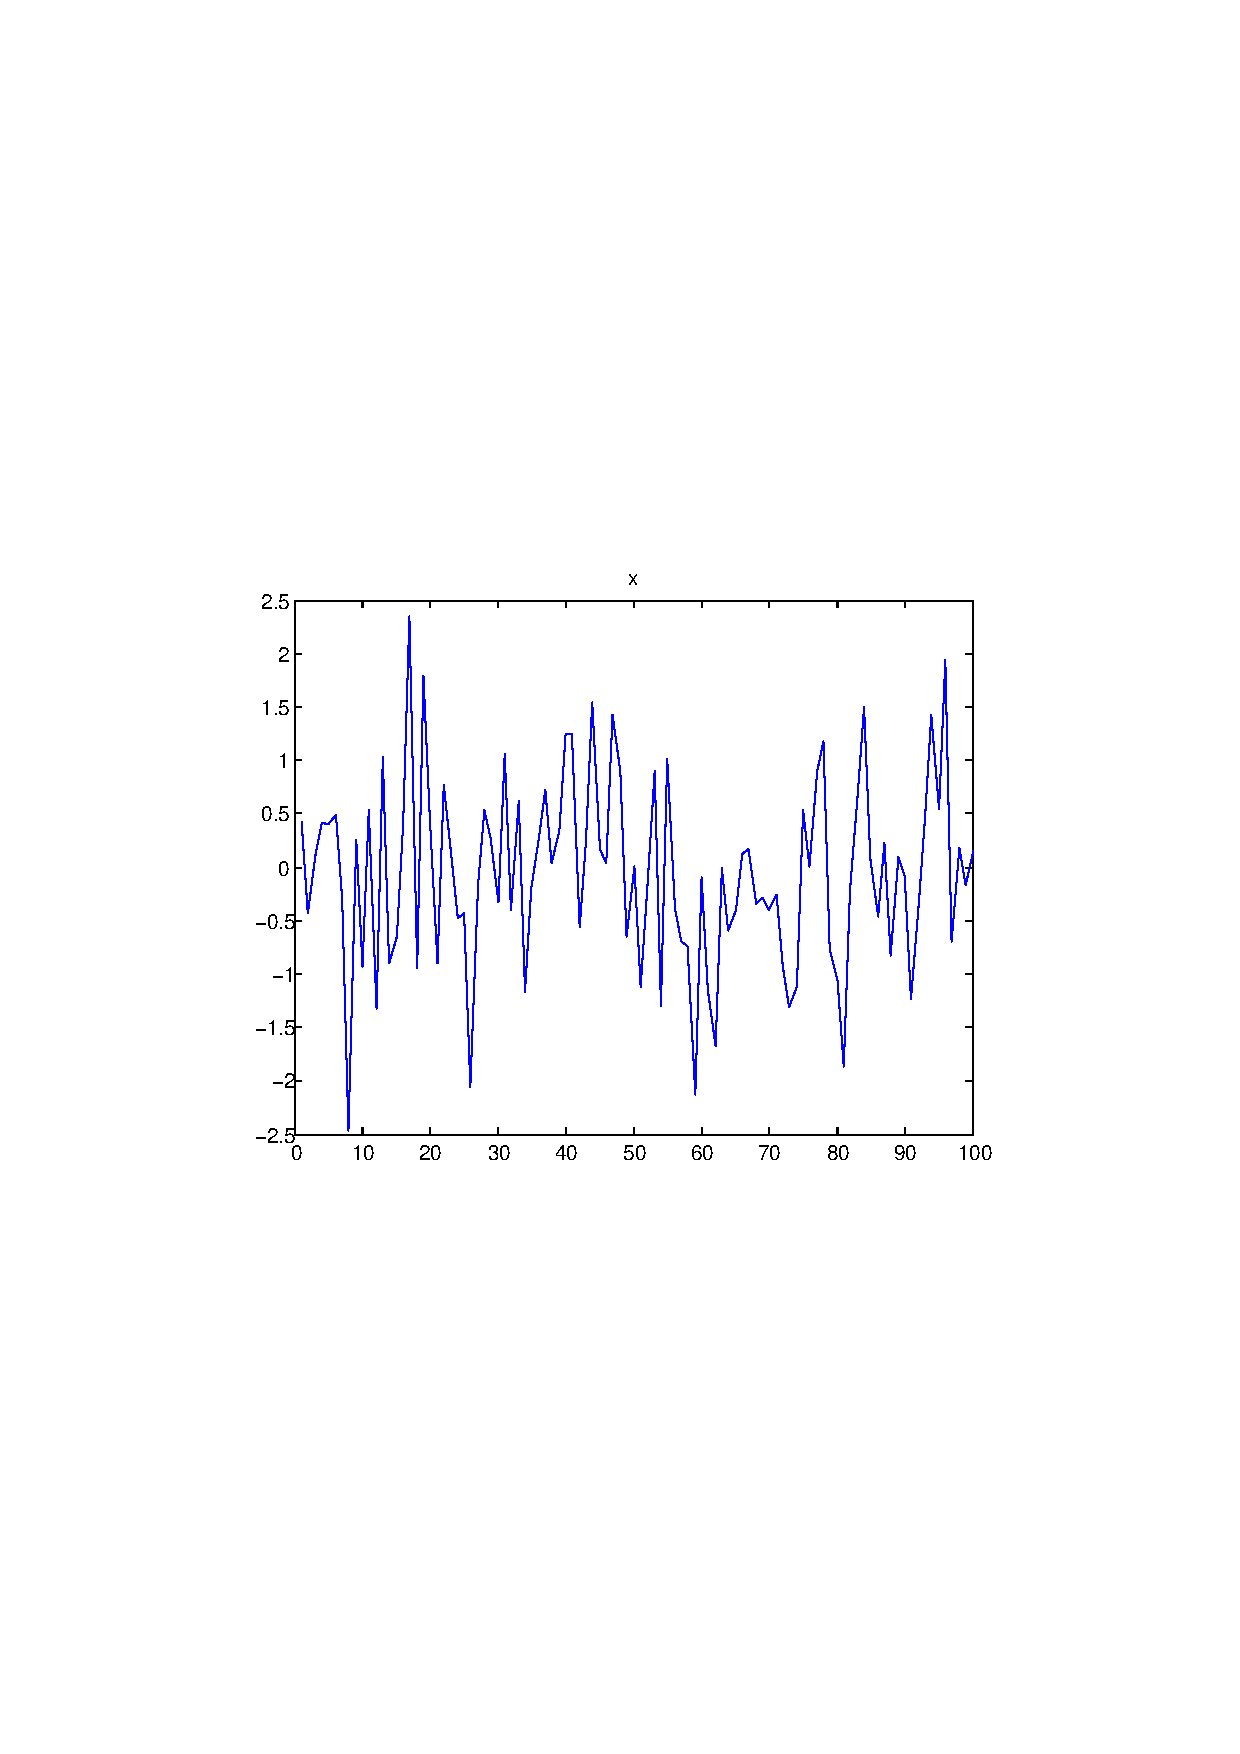
\includegraphics[width=0.35\textwidth]{Grafiken/ARMA1.pdf}
			}
			\subfigure[$\theta_1=(0,0,1)'$]{
				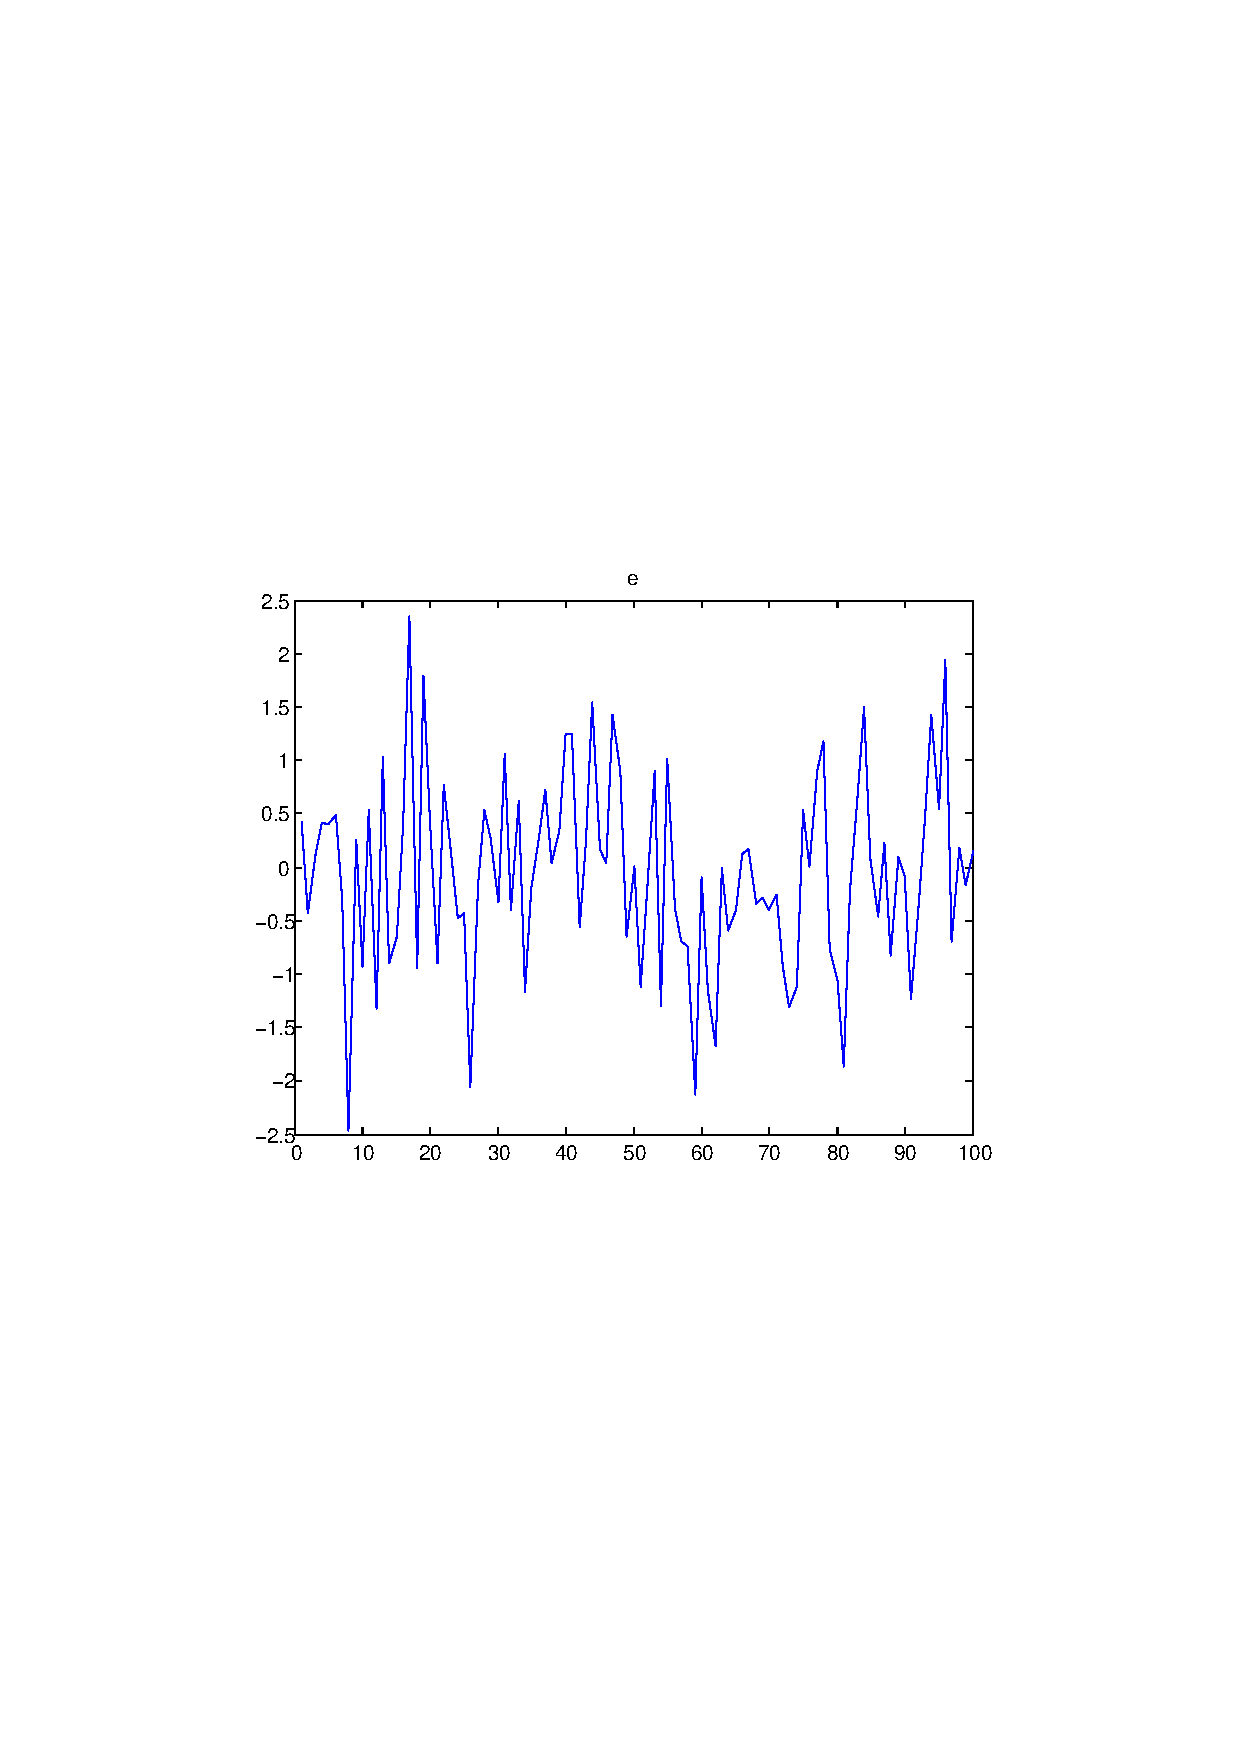
\includegraphics[width=0.35\textwidth]{Grafiken/ARMA2.pdf}
			}
		\end{figure}
		\item Obviously both models generate the same data (as long as the shocks $\varepsilon_t$ are the same). $\theta_0$ and $\theta_1$ are observationally equivalent.
		\item Note $\sigma=1$ is \textbf{partially identifiable}.
	\end{itemize}
\end{frame}


\begin{frame}\frametitle{Identification}
	\begin{itemize}
		\item Identification is a mathematical problem (injectivity).
		\item Identification problems arise if distinct parameter values do not lead to distinct probability distributions of the data.
		\item Drawing inferences from the probability distribution leads thus to wrong conclusions from estimation and inference.
		\item When identification fails, properties of estimators change.
		\item Even with an infinite sample it is not possible to pin down some parameters, no matter what estimation procedure one uses.
		\item Identification tests: Order and rank conditions, via autocovariances, spectral densities, information matrix, imposing restrictions, Bayesian methods \dots can be studied prior to estimation
	\end{itemize}
\end{frame}

\section{References}
\begin{frame}\frametitle{References}
Recommended Readings
  \begin{itemize}
    \item DYNARE USER GUIDE
    \item DeJong/Dave (2011) - Structural Macroeconometrics
    \item An and Schorfheide (2007) - Bayesian Analysis of DSGE Models
  \end{itemize}
\end{frame}




\end{document}
